\documentclass[12pt,a4paper,twopage]{article}
\usepackage[utf8]{inputenc}
\usepackage{geometry}
\geometry{a4paper,left=30mm,right=30mm, top=3cm, bottom=30mm} 
\usepackage{multicol}
\usepackage{amsmath}
\usepackage{float}
\usepackage{epsfig,graphicx}
\usepackage{xcolor,import}
\usepackage{subcaption}
\usepackage[font=small,labelfont=bf]{caption}
\usepackage{siunitx}
\usepackage[german]{babel}
\usepackage{textcomp}
\usepackage{mathtools}
\linespread{1.1}
\usepackage{parskip}
\setlength{\parindent}{12pt}


\begin{document}


\thispagestyle{empty}
			\begin{center}
			\Large{Fakultät für Physik}\\
			\end{center}
\begin{verbatim}


\end{verbatim}
							%Eintrag des Wintersemesters
			\begin{center}
			\textbf{\LARGE SOMMERSEMESTER 2015}
			\end{center}
\begin{verbatim}


\end{verbatim}
			\begin{center}
			\textbf{\LARGE{Physikalisches Praktikum II}}
			\end{center}
\begin{verbatim}




\end{verbatim}

			\begin{center}
			\textbf{\LARGE{PROTOKOLL}}
			\end{center}
			
\begin{verbatim}





\end{verbatim}

			\begin{flushleft}
			\Large{\textbf{Experiment (Nr., Titel):} PS9, Heißluftmotor - Stirlingprozess}\\
			
							%Experiment Nr. und Titel statt den Punkten eintragen
			\LARGE{}	
			\end{flushleft}

\begin{verbatim}

\end{verbatim}	
							%Eintragen des Abgabedatums, oder des Erstelldatums des Protokolls
			\begin{flushleft}
			\textbf{\Large{Datum:}} \Large{29.5.2015}
			\end{flushleft}
			
\begin{verbatim}
\end{verbatim}
							%Namen der Protokollschreiber
		\begin{flushleft}
			\textbf{\Large{Bachleitner Veronika, Grafendorfer Erik}} 
			\end{flushleft}

\begin{verbatim}


\end{verbatim}
							%Kurstag und Gruppennummer, zb. Fr/5
			\begin{flushleft}
			\textbf{\Large{Kurstag/Gruppe:}} \Large{FR/1}
			\end{flushleft}

\begin{verbatim}

\end{verbatim}
							%Name des Betreuers, das Praktikum betreute.
			\begin{flushleft}
			\LARGE{\textbf{Betreuer }:\Large{STANA }}		
			\end{flushleft}
			
\section{Aufgabenstellung}
Wir untersuchen die grundlegenden thermodynamischen Eigenschaften eines Stirlingmotors.
\section{Theorie}
\subsection{Allgemeine Grundlagen}
Es gibt thermodynamische Kreisprozesse, bei denen durch verschiedene Zustandsänderungen einem System Wärme zugeführt oder entnommen wird. Solche Zustandsänderungen sind isotherm (Temperatur konstant), adiabatisch (Wärmemenge konstant) und isochor (Volumen konstant).
\subsubsection{Carnot Prozess}
Eine Carnot-Maschine benützt eine Arbeitssubstanz, mit der sie einen quasistatischen Kreisprozess ausführt:\\
\\
1. Isotherme Zustandsänderung (Expansion). Dabei nimmt as Arbeitsgas die Wärmemenge $Q_{zu}$ auf.\\
2. Adiabatische Zustandsänderung (Expansion). Dabei hat das Arbeitsgas am Ende die Temperatur $T_2$.\\
3. Isothemre Zustandsänderung (Kompression). Dabei gibt as Arbeitsgas die Wärmemenge $Q_{ab}$ ab.\\
4. Adiabatische Zustandsänderung (Kompression). Dabei hat das Arbeitsgas am Ende die Temperatur $T_1$.\\
\\
Technisch ist der Carnot-Prozess jedoch nicht durchführbar, da einerseits die direkte Abfolge dieser Zustandsänderungen nicht realisierbar und andererseits die Prozesse in den meisten Wärmekraftmaschinen nicht reversibel sind.\\
\\
Der Wirkungsgrad ist gegeben durch:
$$\eta=\frac{A}{Q_{zu}}=\frac{Q_{zu}-Q_{ab}}{Q_{zu}}=1-\frac{Q_{ab}}{Q_{zu}}$$
wo $A$ die Arbeit und $Q_{zu}$ bzw. $Q_{ab}$ die zugeführte bzw. abgeführte Wärmemenge sind.\\
\\
Der Stirling-Kreisprozess besteht aus isothermen und isochoren Zustandsänderungen:\\
\\
1. Isotherme Zustandsänderung (Expansion).\\
2. Isochore Zustandsänderung (Expansion).\\
3. Isotherme Zustandsänderung (Kompression).\\
4. Isochore Zustandsänderung (Kompression).\\
\\
Verwendet man die ideale Gasgleichung ($pV=NkT$) sowie die Formeln für die Zustandsänderungen erhält man für den (idealen) Wirkungsgrad:
$$\eta=\frac{T_1-T_2}{T_1}=1-\frac{T_2}{T_1}$$
Dieser wird im Experiment dann auch berechnet mittels:
$$\eta_{ideal}=\frac{P_{ideal}}{P_{zu}}$$
wobei $P_{ideal}$ die Leistung im Leerlauf und $P_{zu}$ die zugeführte Leistung ist.\\
\\
Der reale Wirkungsgrad dagegen ist gegeben durch
$$\eta_{real}=\frac{P_{real}}{P_{zu}}$$
wo $P_{real}$ die Leistung des belasteten Motors ist. Die Leistung kann in unserem ersten Versuch auch über folgendes Skalarprodukt bestimmt werden:
$$P=\vec{M}\cdot\vec{\omega}=\vec{F}\times\vec{r}\cdot\vec{\omega}$$
wo $\vec{M}$ das Bremsdrehmoment, $vec{F}$ die Kraft, $\vec{r}$ der Radius und $\vec{\omega}$ die Winkelgeschwindigkeit ist.\\
\\
Bei der \textit{Stirling-Maschine als Kältemaschine} wird im Prinzip ein Kreisprozess wie der oben beschriebene durchgeführt. Da es sich allerdings um eine Kältemaschine handeln soll, wird der Kreispozess jedoch gegen den Uhrzeigersinn durchlaufen.

\section{Aufbau}
\subsection{Wärmekraftmaschine}
Mit einer Glühwendel wird das Wärmereservoir eines Stirlingmotors erhitzt, dessen Kältereservoir über eine Wasserkühlung bereitgestellt wird. Nach einer kurzen Aufwärmzeit wird ein Schwungrad angeworfen, das über eine Schubkurbel mit Phasenverschiebung zwei Kolben im Stirlingmotor betreibt. Die Phasenverschiebung wird dadurch ermöglicht, dass eine der Triebstangen für die Kolben um einen Viertelkreis verschoben zur anderen am Rand der Schubkurbel angebracht ist. So werden die vier Phasen für den Kreisprozess ermöglicht. 

Die Luft nimmt Wärme von der Glühwendel auf und das Volumen im Zylinder wird zugleich vergrößert, wodurch sich seine Temperatur nicht ändert, dann schiebt der Verdrängerkolben heiße Luft zum Kältereservoir, dort wird die Luft abgekühlt und der Druck sinkt, dann komprimiert der zweite Kolben die Luft, wodurch der Druck steigt, durch die Kühlung aber wieder die Temperatur konstant bleibt, und schließlich saugt der Verdrängerkolben wieder heiße Luft nach und das Volumen wird wieder vergrößert. 

Werden die Bewegungen, die durch das Verschieben der beiden Kolben von alleine entstehen, miteinander gekoppelt und der Prozess über ein Schwungrad in Gang gesetzt, kann sich der Prozess mit der ihm zugeführten Wärme von alleine in Gang halten - ein Kreisprozess entsteht.

Wir messen die elektrische Leistung, die von der Glühwendel abgegeben wird, und die mechanische Leistung, die der Motor durch sie leistet.


\subsection{Kältemaschine}
Bei der Kältemaschine wird die umgekehrte Richtung betrachtet - wenn man die mechanischen Bewegungen erzwingt, wird durch die Kompression, den Lufftransport und durch die Relaxation Wärme von einem zum anderen Reservoir transportiert. Wir haben einen Kühlschrank, dessen Kühlleistung wir messen.


\section{Durchführung}

\subsection{Wärmekraftmaschine}
Es wird ein Stroboskop ($\pm 0.01$) Hz verwendet, um die Drehzahl zu messen, ein Prony'scher Bremszaun zusammen mit einer Federwaage von ($(1 \pm 0.01)$N, ein Multimeter zur Leistungsmessung an der Glühwendel, sowie ein extenes Sensorcassy für die Druck und Volumsmessung im Zylinder, das an einen Computer angeschlossen ist.
\subsection{Kältemaschine}
Wir verwenden zusätzlich einen externen Motor, der über einen Keilriemen das Schwungrad des Stirlingmotors antreibt - wieder messen wir die Drehzahl mit dem selben Stroboskop und bestimmen zusätzlich die Leistung des Motors mit einem Multimeter und die Temperatur im Zylinder mit einem Sensor Cassy.
\section{Ergebnisse}
\subsection{Wärmekraftmaschine}

\begin{center}
\begin{figure}[H]
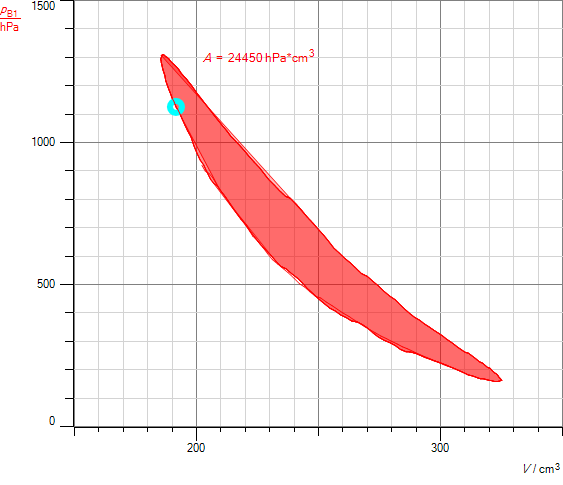
\includegraphics[scale=0.7]{bachgraf/heissluft.png}
\caption{P-V-Diagramm der Wärmekraftmaschine mit angegebener Arbeit (Flächeninhalt).}
\label{fig:heissluft-pv}
\end{figure}
\end{center}

In Abbildung \ref{fig:heissluft-pv} ist das P-V-Diagramm der Wärmekraftmaschine zu sehen. Die Fläche unter der Kurve, und damit die Arbeit, wird vom Programm berechnet als:
$$A=24450hPa cm^3 =(2.445 \pm 0.001) Ws$$

Mit dem Stroboskop kann die Leerlauf-Frequenz gemessen werden:

$$f_0=(5.26 \pm 0.01)Hz$$

Wenn wir die mechanische Arbeit mit der Leerlauf-Frequenz $f_0$ multiplizieren erhalten wir die ideale Leistung des Motors:

$$\boxed{P_{ideal}=(12.861 \pm 0.025)W}$$

Die zugeführte Leistung ergibt sich aus folgenden Strom- bzw. Spannungswerten: 

$U=(11 \pm 1)V$, $I=(13 \pm 1)A$
$$\boxed{P_{zu}=U \cdot I = (143 \pm 17)W}$$

Die Unsicherheit der zugeführten Leistung ergibt sich aus:

$\sqrt{(U\cdot\Delta I)^2+(I\cdot\Delta U)^2}=\sqrt{11^2+13^2}\approx17.029$

Aus der idealen und der zugeführten Leistung können wir den idealen Wirkungsgrad berechnen:

$$\boxed{\eta_{ideal}=\frac{P_{ideal}}{P_{zu}}=(9.0 \pm 0.1)\%}$$

Als nächstes wird der reale Wirkungsgrad des Motors bestimmt, indem wir mit dem Prony'schen Bremszaum eine Leistung unter Belastung abnehmen.

Wir stellen anhand der Federwaage folgende Bremskraft fest:
$$F=(0.62-0.16 \pm 0.01)N=(0.46 \pm 0.01)N$$
wobei die abgezogenen $0.16$ den Nullpunkt auf der Federwaage markieren.

Die Frequenz war dabei
$$f=(4.29 \pm 0.01)Hz$$

Den Radius des Bremszaums haben wir nicht selbst gemessen aber bei Mitstudenten erfragt: $r=(0.250 \pm 0.002)m$

Aus diesen drei Werten können wir uns den realen Wirkungsgrad berechnen.

Das Bremsdrehmoment ist $\vec{M}=\vec{F}\times \vec{r}=F\cdot r = (0.115 \pm 0.003)Nm$ und die reale Leistung is daraus:
$$\boxed{P_{real}=M\cdot f=(0.49 \pm 0.01)W}$$

Daraus erhalten wir schließlich den realen Wirkungsgrad:
$$\boxed{\eta_{real}=\frac{P_{real}}{P_{zu}}=(0.35 \pm 0.05)\%}$$

Der Wirkungsgrad des Motors ist:

$$\eta_{Motor}=\frac{P_{real}}{\int pdV \cdot f} = \frac{0.49W}{12.86W} $$

$$\boxed{ \eta_{Motor}=(3.81 \pm 0.01) \% }$$
\subsection{Kältemaschine}

\begin{center}
\begin{figure}[H]
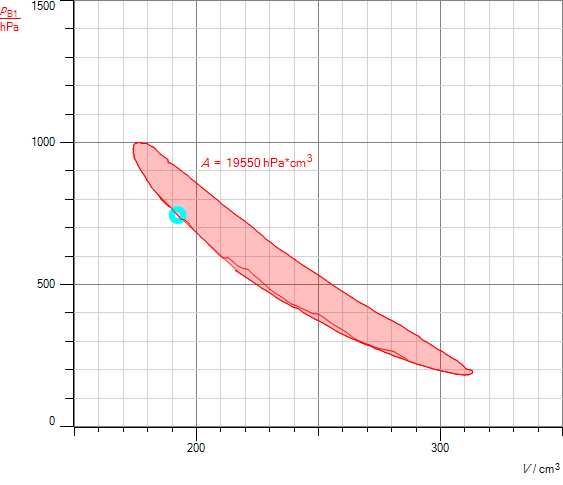
\includegraphics[scale=0.7]{bachgraf/kaeltemaschine.png}
\label{kaeltemaschine-pv}
\caption{Arbeit der Kältemaschine}
\end{figure}
\end{center}

Erste Messung:

$8.2^\circ C$ bei $(350 \pm 10)mA$ und $(240 \pm 10)V$\\
Heizleistung: $(7.0 \pm 0.5)V$ $(1.5 \pm 0.1)A$

Zweite Messung:

$8.0^\circ C$ bei $(350 \pm 10)mA$ und $(240 \pm 10)V$ am externen Motor\\
Heizleistung: $(8.0 \pm 0.5)V$ $(1.7 \pm 0.1)A$ \\
Frequenz: $f=4.63Hz$

Wir erhalten für die erste Messung einen realen Wirkungsgrad der Kühlmaschine von 

$$\eta_{real} = \frac{P_{Kuehl} }{P_{Extern} } = \frac{7.0 V \cdot 1.5 A}{0.350 A \cdot 240 V}$$

$$\boxed{ \eta_{real}=(12.5 \pm 1.5) \% }$$ 

\section{Diskussion}
\subsection{Wärmekraftmaschine}
Der reale Wirkungsgrad des Stirlingmotors ist mit unter einem Prozent sehr klein, aber glaubhaft, da es nicht nur ein generell ineffizienter Motor ist - der ideale Wirkungsgrad liegt bei 10\%! - sondern die Leistung sehr ineffizient abgegriffen wird - allein über die Reibung am Holz des Prony'schen Bremszauns wird ein Drehmoment erzeugt, während sich unter ihm die Achse weiter dreht und der Großteil der Leistung weiter in Rotation des Schwungrades investiert wird. Zusätzlich geht viel Enerige in Reibungswärme verloren. 
\subsection{Kältemaschine}
Durch die schlechte Isolation des Zylinders wird er natürlich dauernd von der Umgebung erwärmt, wodurch die eigentliche Kühlleistung des Stirlingmotors als geringer gemessen wird, als sie eigentlich ist. 																						
\end{document}